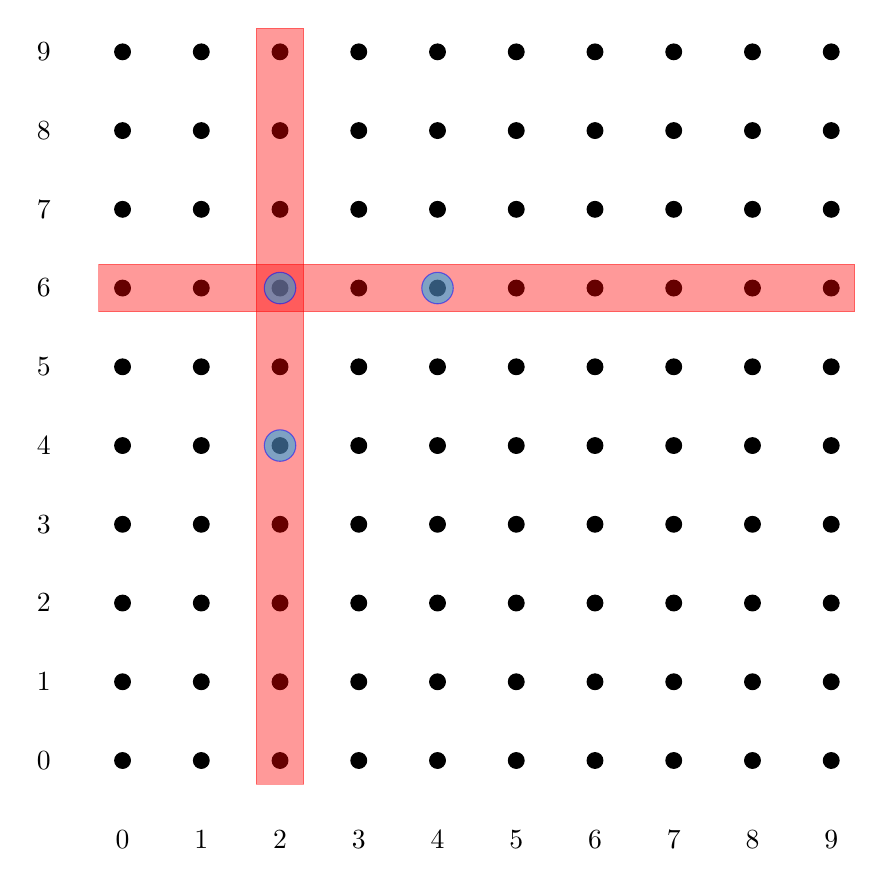
\begin{tikzpicture}
    \foreach\x in {0,1,2,3,4,5,6,7,8,9}{
        \foreach\y in {0,1,2,3,4,5,6,7,8,9}{
            \draw[fill=black] (\x,\y) circle (0.1);
        }
        \node at (\x, -1) {$\x$};
        \node at (-1, \x) {$\x$};
    }

    \draw[fill=red,draw=red,opacity=0.4] ( 1.7, -0.3) rectangle (2.3, 9.3);
    \draw[fill=red,draw=red,opacity=0.4] (-0.3,  5.7) rectangle (9.3, 6.3);

    \draw[draw=blue,fill=cyan,opacity=0.5] (2, 4) circle (0.2);
    \draw[draw=blue,fill=cyan,opacity=0.5] (4, 6) circle (0.2);
    \draw[draw=blue,fill=cyan,opacity=0.5] (2, 6) circle (0.2);
\end{tikzpicture}